% !TEX program = xelatex

\documentclass[screen,17pt,cn,founder,mtpro2]{elegantnote}

\usepackage{subcaption}
\title{基于深度学习的行为识别数据分析 \\ ------\large{ “深度学习入门及 Python 训练” 课程报告}}
\author{龚梓阳}
\date{\zhtoday}

\begin{document}

\maketitle
\clearpage

\section{数据介绍}

% 该实验在 30 位年龄在 19\~48 岁的志愿者中进行,每一位志愿者会在腰部佩戴智能手机(Samung Galaxy S II),要求志愿者在指定时间内按照其使用习惯完成指定动作(步行,上楼,下楼,坐,站与躺),并基于智能手机的嵌入式加速度计与陀螺仪,以 50 Hz 的恒定速率记录 3 轴线性加速度与角速度。

\begin{figure}[hpt]
    \centering
    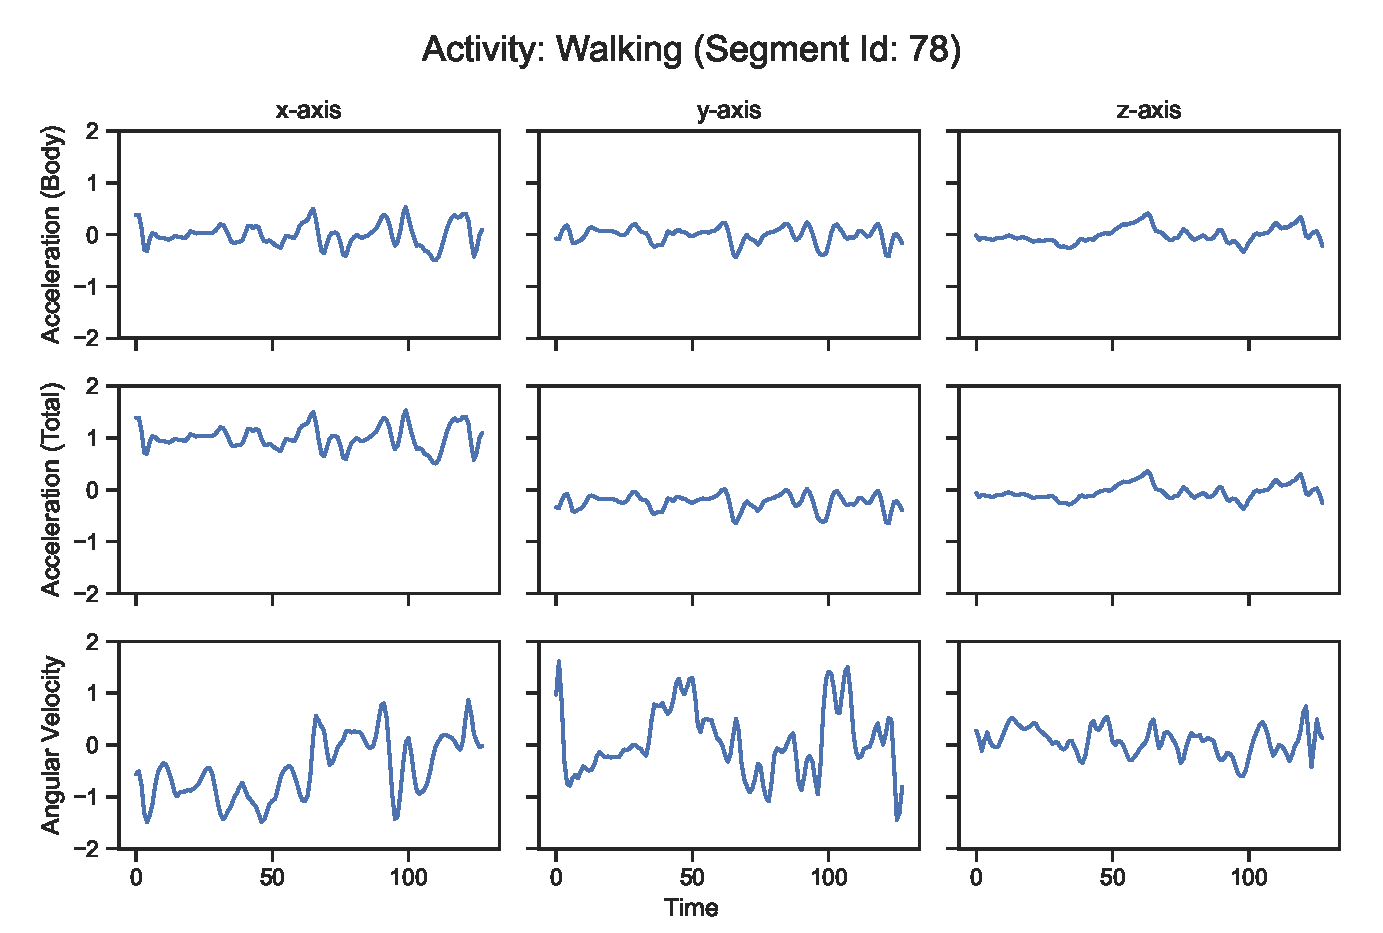
\includegraphics[width=.7\linewidth]{images/activity-walking-segment-78.eps}
    \caption{指定时间内完成指定行为(步行)的智能手机传感器数据记录}
\end{figure}

\begin{figure}
    \begin{subfigure}{.33\textwidth}
        \centering
        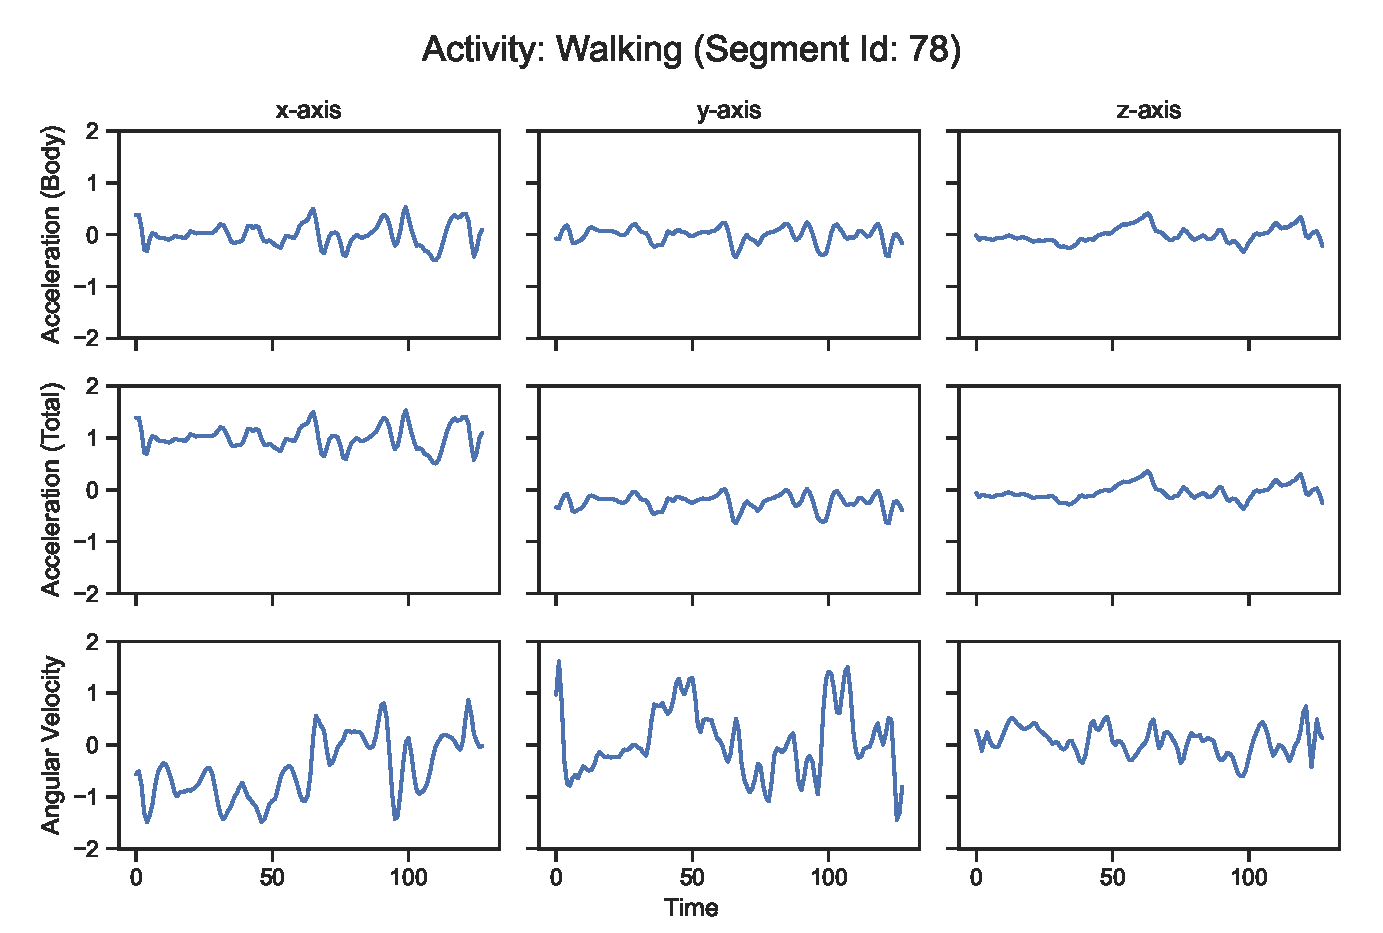
\includegraphics[width=\linewidth]{images/activity-walking-segment-78.eps}
        \caption{步行}
    \end{subfigure}
    \begin{subfigure}{.33\textwidth}
        \centering
        \includegraphics[width=\linewidth]{images/activity-upstairs-segment-150.eps}
        \caption{上楼}
    \end{subfigure}
    \begin{subfigure}{.33\textwidth}
        \centering
        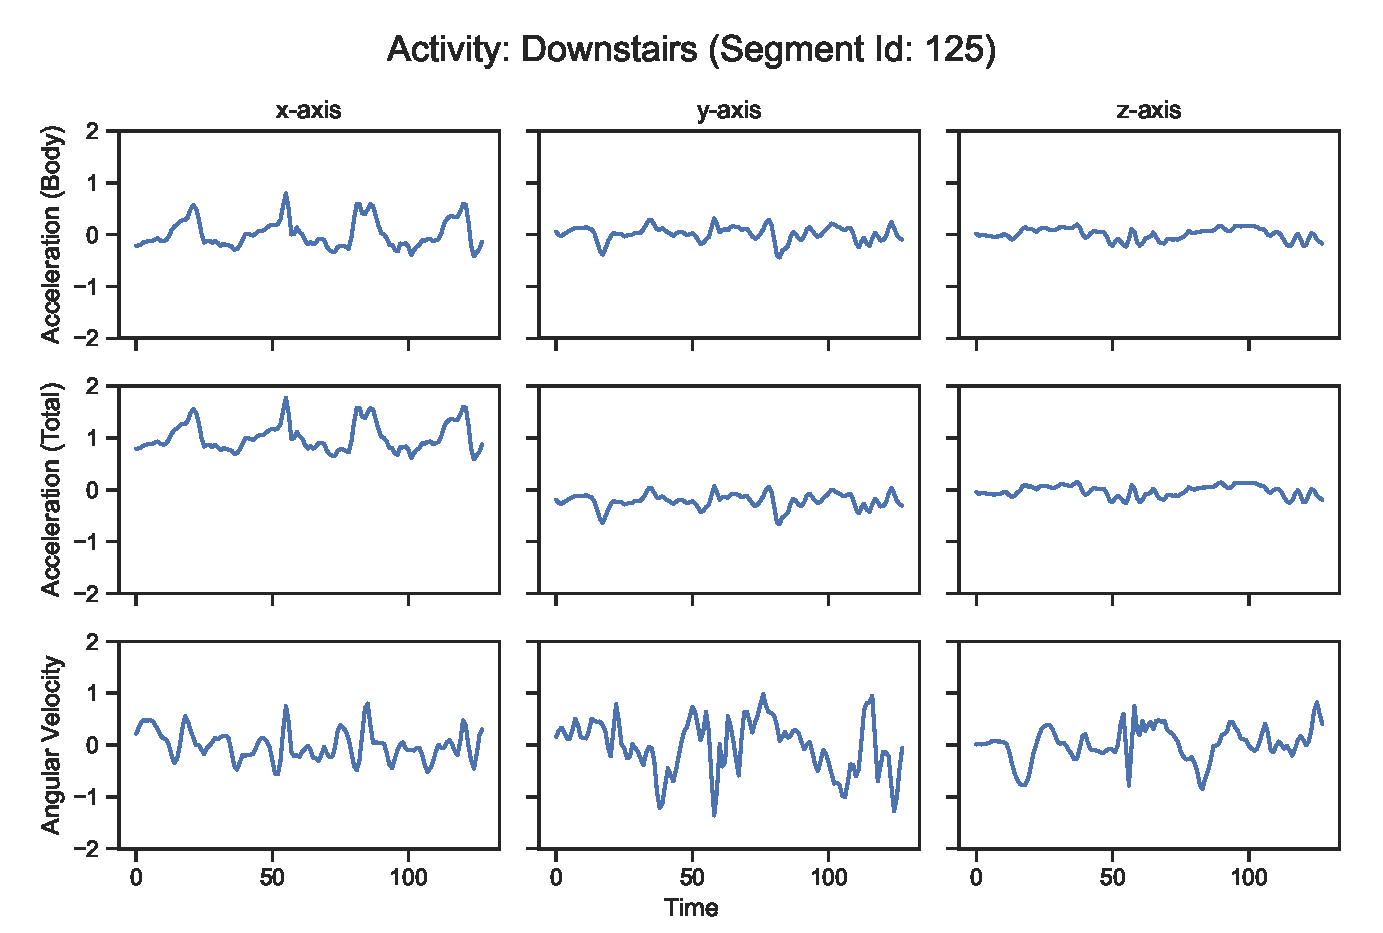
\includegraphics[width=\linewidth]{images/activity-downstairs-segment-125.eps}
        \caption{下楼}
    \end{subfigure}
    \begin{subfigure}{.33\textwidth}
        \centering
        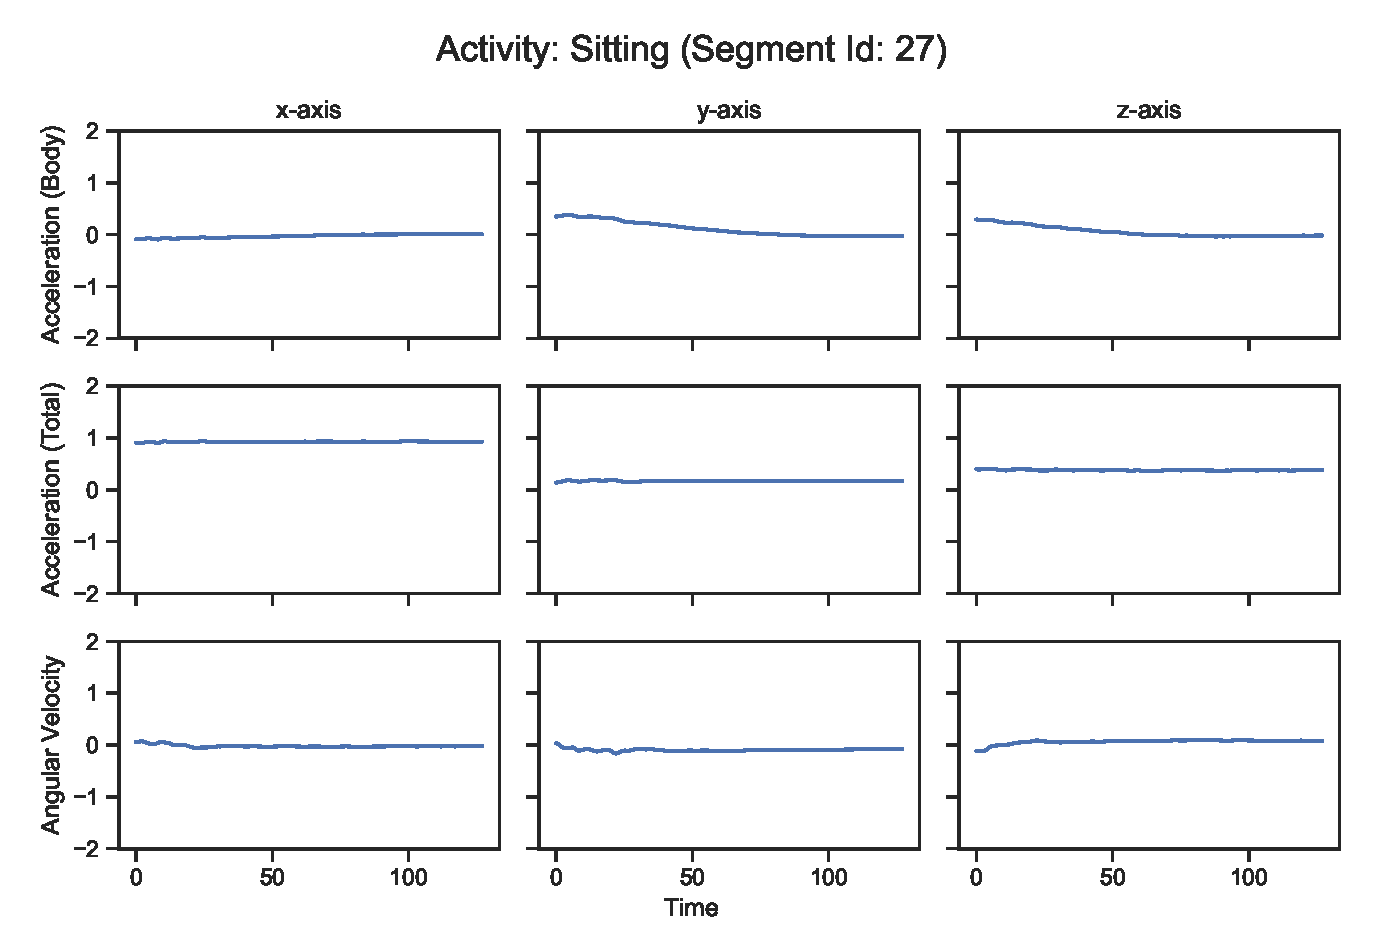
\includegraphics[width=\linewidth]{images/activity-sitting-segment-27.eps}
        \caption{静坐}
    \end{subfigure}
    \begin{subfigure}{.33\textwidth}
        \centering
        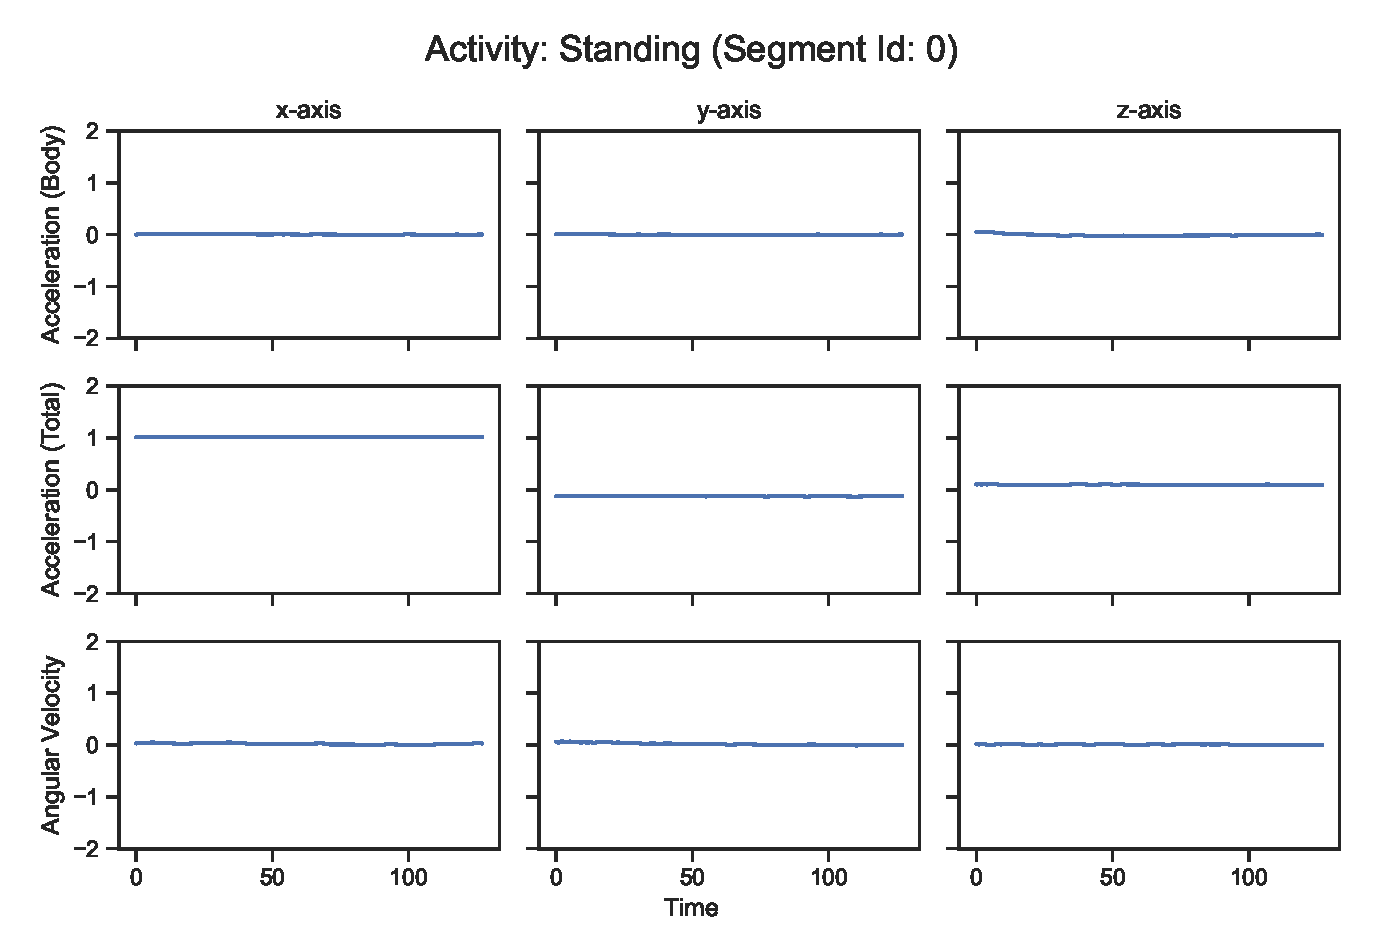
\includegraphics[width=\linewidth]{images/activity-standing-segment-0.eps}
        \caption{站立}
    \end{subfigure}
    \begin{subfigure}{.33\textwidth}
        \centering
        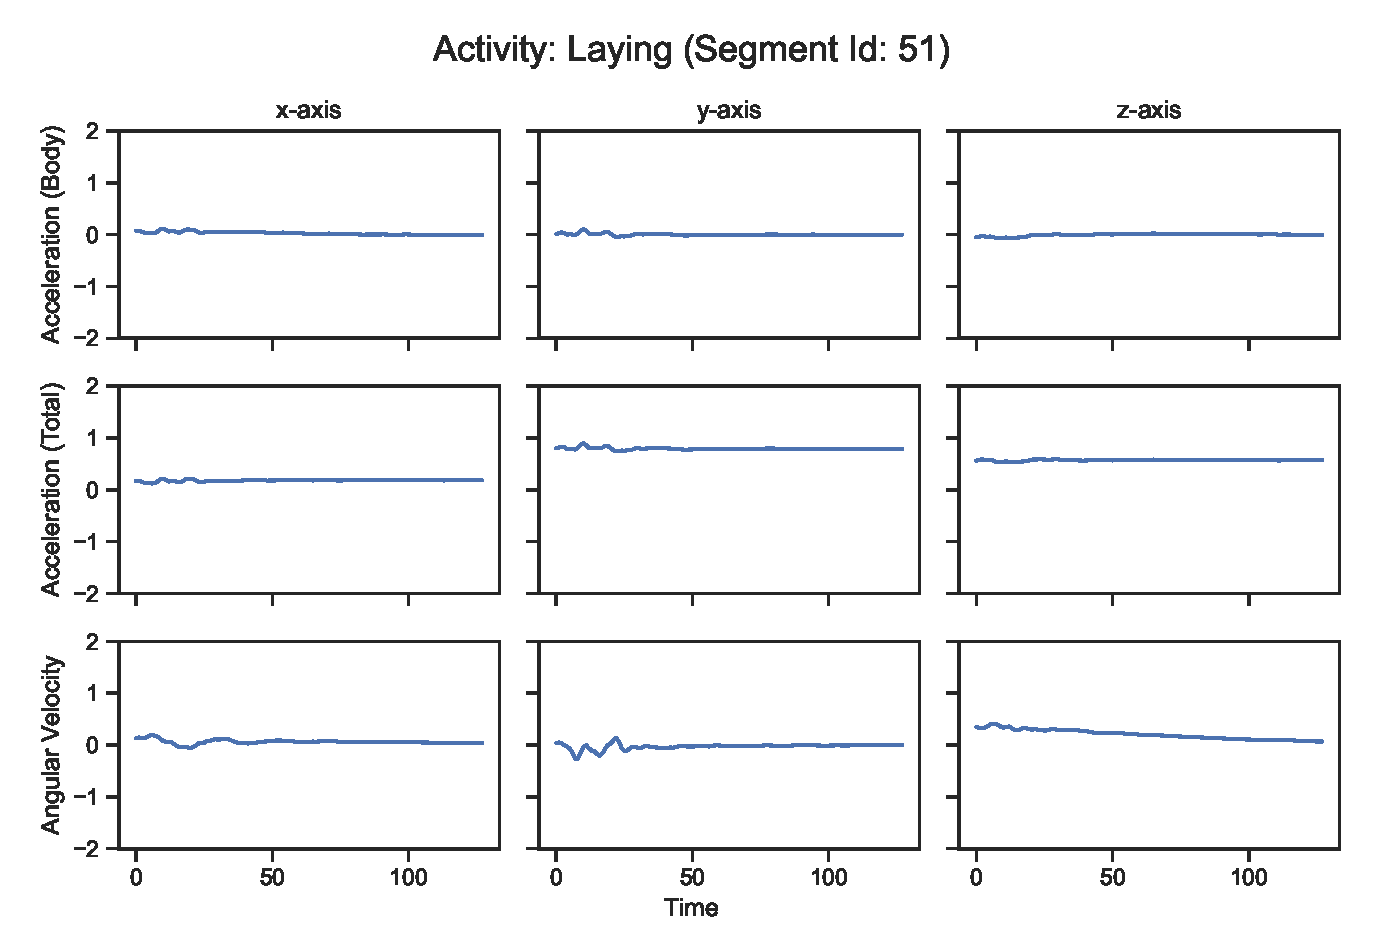
\includegraphics[width=\linewidth]{images/activity-laying-segment-51.eps}
        \caption{平躺}
    \end{subfigure}
    \caption{指定时间内完成不同指定行为(步行,上楼,下楼,静坐,站立和平躺)的智能手机传感器数据记录}
\end{figure}
\clearpage

\section{模型构建}

\subsection{基于统计特征的机器学习模型}

根据 ??? 工作中所构建的 561 个基于时域特征及频域特征的变量,包括采用多种滤波器及快速傅里叶变换所构建的统计特征。

\paragraph{随机森林}

\paragraph{AdaBoost}

\paragraph{支持向量机}

\clearpage

\subsection{基于 LSTM 的深度学习模型}


\clearpage

\section{结果总结}

\end{document}